% Warburg Effect: Normal vs Cancer Cell Metabolism
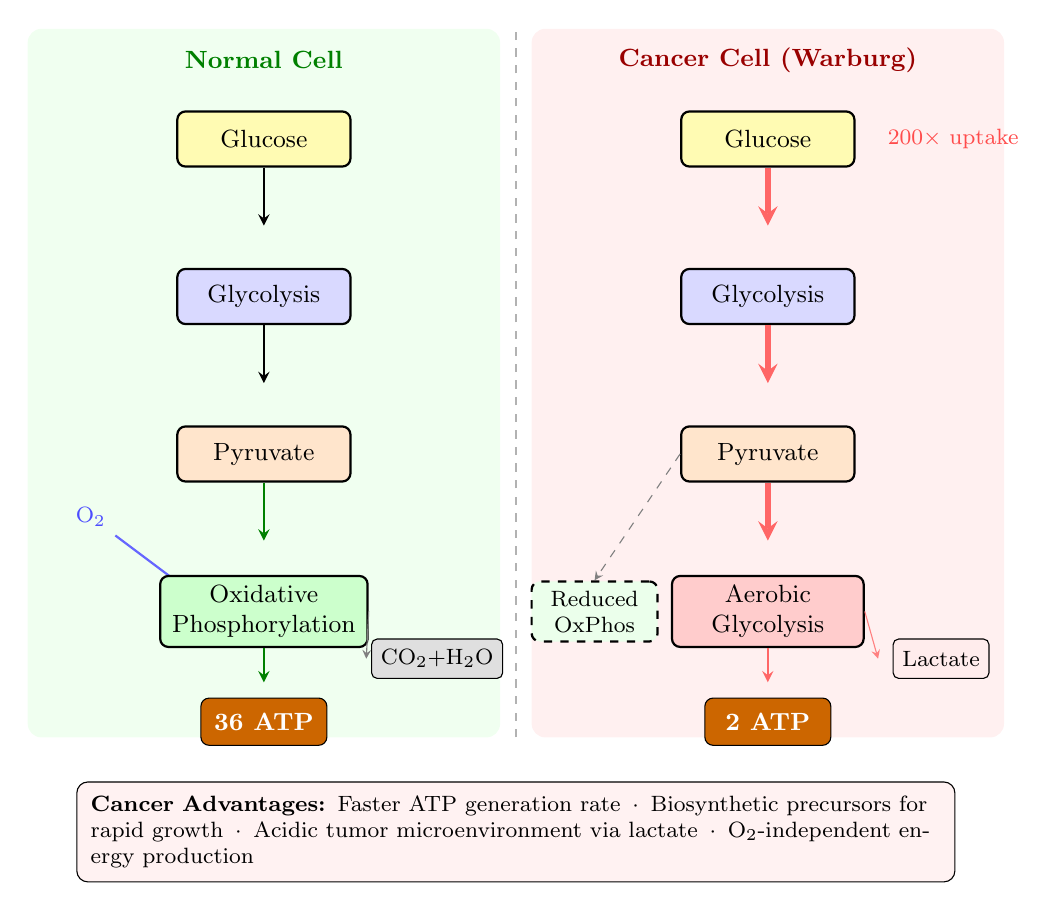
\begin{tikzpicture}[
  box/.style={draw, rounded corners=3pt, minimum width=2.2cm, minimum height=0.7cm,
              align=center, font=\small, thick},
  atp/.style={draw, rounded corners=3pt, font=\small\bfseries, text=white, fill=orange!80!black,
              minimum width=1.6cm, minimum height=0.6cm, align=center},
  byproduct/.style={draw, rounded corners=2pt, font=\footnotesize, fill=gray!25,
                    minimum height=0.5cm, align=center},
  arrow/.style={->, >=stealth, thick},
  fatarrow/.style={->, >=stealth, line width=2pt},
]

% Background panels
\fill[green!6, rounded corners=5pt] (-3.2, -0.4) rectangle (2.8, 8.6);
\fill[red!6, rounded corners=5pt] (3.2, -0.4) rectangle (9.2, 8.6);

% Panel headers
\node[font=\small\bfseries, green!50!black] at (-0.2, 8.2) {Normal Cell};
\node[font=\small\bfseries, red!60!black] at (6.2, 8.2) {Cancer Cell (Warburg)};

% Dividing line
\draw[dashed, gray!60, thick] (3.0, -0.4) -- (3.0, 8.6);

% === Normal Cell (left column, centered at x=0) ===
\node[box, fill=yellow!30] (gn) at (-0.2, 7.2) {Glucose};
\draw[arrow] (gn) -- ++(0, -1.1);

\node[box, fill=blue!15] (gly_n) at (-0.2, 5.2) {Glycolysis};
\draw[arrow] (gly_n) -- ++(0, -1.1);

\node[box, fill=orange!20] (pyr_n) at (-0.2, 3.2) {Pyruvate};
\draw[arrow, green!50!black] (pyr_n) -- ++(0, -1.1);

% O2 input
\node[font=\footnotesize, blue!70] (o2) at (-2.4, 2.4) {O$_2$};
\draw[arrow, blue!60] (o2) -- (-1.2, 1.5);

\node[box, fill=green!20, text width=2.4cm] (oxphos) at (-0.2, 1.2) {Oxidative\\Phosphorylation};
\draw[arrow, green!50!black] (oxphos) -- ++(0, -0.9);

\node[atp] (atp_n) at (-0.2, -0.2) {36 ATP};

\node[byproduct] at (2.0, 0.6) {CO$_2$+H$_2$O};
\draw[->, >=stealth, thin, gray] (oxphos.east) -- (1.1, 0.6);

% === Cancer Cell (right column, centered at x=6.2) ===
\node[box, fill=yellow!30] (gc) at (6.2, 7.2) {Glucose};
\node[font=\footnotesize, red!70, right] at (7.6, 7.2) {200$\times$ uptake};
\draw[fatarrow, red!60] (gc) -- ++(0, -1.1);

\node[box, fill=blue!15] (gly_c) at (6.2, 5.2) {Glycolysis};
\draw[fatarrow, red!60] (gly_c) -- ++(0, -1.1);

\node[box, fill=orange!20] (pyr_c) at (6.2, 3.2) {Pyruvate};
\draw[fatarrow, red!60] (pyr_c) -- ++(0, -1.1);

\node[box, fill=red!20, text width=2.2cm] (aero) at (6.2, 1.2) {Aerobic\\Glycolysis};
\draw[arrow, red!60] (aero) -- ++(0, -0.9);

\node[atp] (atp_c) at (6.2, -0.2) {2 ATP};

% Lactate
\node[byproduct, fill=pink!30] (lac) at (8.4, 0.6) {Lactate};
\draw[->, >=stealth, thin, red!50] (aero.east) -- (7.6, 0.6);

% Dashed branch to reduced OxPhos
\node[box, fill=green!8, font=\footnotesize, dashed, minimum width=1.6cm] (rox) at (4.0, 1.2) {\footnotesize Reduced\\OxPhos};
\draw[->, >=stealth, dashed, gray] (pyr_c.west) -- (rox.north);

% === Bottom advantages box (full width) ===
\node[draw, rounded corners=4pt, fill=red!5, text width=10.8cm, align=left, font=\footnotesize,
      inner sep=5pt] at (3.0, -1.6) {%
\textbf{Cancer Advantages:}\enspace
Faster ATP generation rate \,$\cdot$\,
Biosynthetic precursors for rapid growth \,$\cdot$\,
Acidic tumor microenvironment via lactate \,$\cdot$\,
O$_2$-independent energy production};

\end{tikzpicture}
